\section{Background \& Methodology}

\subsection{CNRS Benchmark}

The CNRS benchmark \cite{tiberga_results_2020} consists of three
\textit{Phases} and
eight \textit{Steps} in total. Each step is a well-defined subproblem for
systematically assessing \gls{MSR} software capabilities and pinpointing
the source of discrepancies between software. Phase 0 consists of
single-physics problems in fluid dynamics, neutronics, and temperature,
respectively. Phase 1 consists of coupled, steady-state eigenvalue problems.
Lastly, Phase 2 consists of a coupled, transient scenario. Table
\ref{table:benchmark} provides brief descriptions of each step, except for the
last transient case as it is still a work in progress at the time of writing.

The domain geometry is a 2m by 2m square cavity filled with LiF-BeF$_2$-UF$_4$
molten salt at an initial temperature of 900K \cite{tiberga_results_2020}.
Standard vacuum boundary conditions apply for neutron flux along the
boundaries, with homogeneous boundary conditions for delayed neutron
precursors. No-slip boundary conditions apply for flow in the cavity, except
the top boundary when the subproblem imposes forced convection via lid-driven
cavity flow. For temperature, all boundaries are insulated and we simulate salt
cooling with the following volumetric heat sink equation:
%
\begin{align}
    q'''(\vec{r}) &= \gamma \left(900 - T(\vec{r})\right), \label{eq:heat}
    \intertext{where}
    q''' &= \mbox{volumetric heat sink [W$\cdot$m$^{-3}$],}
    \nonumber \\
    \gamma &= \mbox{heat transfer coefficient [W$\cdot$m$^{-3}\cdot$K$^{-1}$],}
    \nonumber \\
    T(\vec{r}) &= \mbox{temperature at point $(\vec{r})$ [K].} \nonumber
\end{align}

Tiberga et al. \cite{tiberga_results_2020} used Serpent 2
\cite{leppanen_serpent_2014} with the JEFF-3.1 library
\cite{koning_jeff-31_2006} to generate multigroup neutronics data for the
LiF-BeF$_2$-UF$_4$ salt in the domain at 900K. They condensed the neutronics
data into six energy groups and eight precursor groups. Their paper contains
all relevant data \cite{tiberga_results_2020}. The benchmark prescribes the
following equations to govern the temperature dependence in the cross sections
and the neutron diffusion coefficients:
%
\begin{align}
    \Sigma_i (T) &= \Sigma_i(T_{ref})
    \frac{\rho_{fuel}(T)}{\rho_{fuel}(T_{ref})}, \\
    D (T) &= D(T_{ref})
    \frac{\rho_{fuel}(T_{ref})}{\rho_{fuel}(T)},
    \intertext{where}
    \Sigma_i &= \mbox{relevant macroscopic cross section [cm${-1}$],}
    \nonumber \\
    D &= \mbox{neutron diffusion coefficient [cm$^2\cdot$s$^{-1}$],}   
    \nonumber \\
    \rho_{fuel} &= \mbox{density of the fuel salt [kg$\cdot$m$^{-3}$],}
    \nonumber \\
    T_{ref} &= \mbox{reference temperature} = 900\mbox{ K}. \nonumber
\end{align}

The benchmark also prescribes for incompressible Navier-Stokes and the
Boussinesq approximation for buoyancy when evaluating the salt flow in the
domain but places no restrictions on the type of neutronics model.

\begin{table*}[t!]
	\caption{Description of each benchmark subproblem.}
	\centering
	\small
	\setlength\tabcolsep{2.5pt}
	\begin{tabular}{p{33mm} p{65mm} l p{40mm}<{\centering}}
		\toprule
		Step & Description & Input parameters & Observables \\
		\midrule
		Step 0.1: Velocity field & Solve for the steady-state incompressible
		flow solution from lid-driven cavity flow. &
		$\begin{aligned}[t]
		    U_{lid} &= 0.5 \mbox{ m$\cdot$s$^{-1}$}
        \end{aligned}$
        & $(u_x, u_y)$ along AA' and BB'; \\
        \midrule
        Step 0.2: Neutronics & Solve for the fission rate density
        $\sum^G_i \Sigma_{f,i} \phi_i(\vec{r})$ and reactivity $\rho$
        in a static, isothermal fuel configuration. &
		$\begin{aligned}[t]
		    U_{lid} &= 0 \mbox{ m$\cdot$s$^{-1}$} \\
		    T &= 900 \mbox{ K} \\
		    P &= 1 \mbox{ GW}
        \end{aligned}$
        & $\sum^G_i \Sigma_{f,i} \phi_i(\vec{r})$ along AA'; \newline
        $\rho$; \\
        \midrule
        Step 0.3: Temperature & Solve for the temperature distribution $T$
        arising from the velocity field $(u_x, u_y)_{s_{0.1}}$ and fission heat
        generation $Q_{s_{0.2}}$ from Steps
        0.1 and 0.2, respectively, and a volumetric heat sink (Equation
        \ref{eq:heat}). &
		$\begin{aligned}[t]
		    (u_x, u_y) &= (u_x, u_y)_{s_{0.1}} \\
		    Q &= Q_{s_{0.2}} \\
		    \gamma &= 10^6 \mbox{ W$\cdot$m$^{-3}\cdot$K$^{-1}$}
        \end{aligned}$
        & $T$ along AA' and BB'; \\
        \midrule
        Step 1.1: Circulating fuel & Solve for the delayed neutron source
        distribution $\sum_j \lambda_j C_j$ and reactivity $\rho$ in a
        non-static, isothermal fuel configuration. &
		$\begin{aligned}[t]
		    (u_x, u_y) &= (u_x, u_y)_{s_{0.1}} \\
		    T &= 900 \mbox{ K} \\
		    P &= 1 \mbox{ GW}
        \end{aligned}$
        & $\sum_j \lambda_j C_j$ along AA' and BB'; \newline $\rho -
        \rho_{s_{0.2}}$; \\
        \midrule
        Step 1.2: Power coupling & Solve for the temperature distribution $T$,
        reactivity $\rho$, and fission rate density
        $\sum^G_i \Sigma_{f,i} \phi_i(\vec{r})$ under the fixed velocity field
        from Step 0.1. &
		$\begin{aligned}[t]
		    (u_x, u_y) &= (u_x, u_y)_{s_{0.1}} \\
		    P &= 1 \mbox{ GW} \\
		    \gamma &= 10^6 \mbox{ W$\cdot$m$^{-3}\cdot$K$^{-1}$}
        \end{aligned}$
        & $T$ along AA' and BB'; \newline $\rho - \rho_{s_{1.1}}$; \newline
        $\sum^G_i \Sigma_{f,i} \phi_i(\vec{r}) -
        \left[\sum^G_i \Sigma_{f,i} \phi_i(\vec{r})\right]_{s_{0.2}}$; \\
        \midrule
        Step 1.3: Buoyancy & Solve for the velocity components $(u_x, u_y)$,
        temperature distribution $T$, delayed neutron source
        distribution $\sum_j \lambda_j C_j$, and
        reactivity $\rho$ in a fully coupled system. &
		$\begin{aligned}[t]
		    P &= 1 \mbox{ GW} \\
		    U_{lid} &= 0 \mbox{ m$\cdot$s$^{-1}$} \\
		    \gamma &= 10^6 \mbox{ W$\cdot$m$^{-3}\cdot$K$^{-1}$}
        \end{aligned}$
        & $(u_x, u_y)$ along AA' and BB'; \newline $T$ along AA' and BB';
        \newline $\sum_j \lambda_j C_j$ along AA' and BB'; \newline
        $\rho - \rho_{s_{0.2}}$; \\
        \midrule
        Step 1.4: Full coupling & Solve for the
        reactivity $\rho$ in a fully coupled system with external
        momentum-driven flow and buoyancy effects and various permutations of
        $P$ and $U_{lid}$ values.  &
		$\begin{aligned}[t]
		    \gamma &= 10^6 \mbox{ W$\cdot$m$^{-3}\cdot$K$^{-1}$} \\
		    P &= [0, 1] \mbox{ GW} \\
		    U_{lid} &= [0, 0.5] \mbox{ m$\cdot$s$^{-1}$}
        \end{aligned}$
        & $\rho - \rho_{s_{0.2}}$; \\
		\bottomrule
	\end{tabular}
	\label{table:benchmark}
\end{table*}
%
\begin{figure}[H]
  \centering
  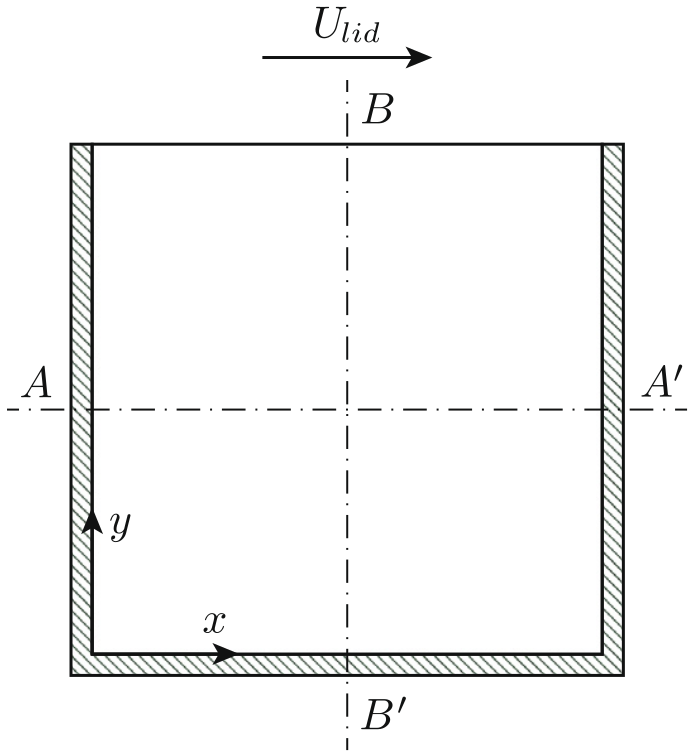
\includegraphics[width=0.75\columnwidth]{domain}
  \caption{The CNRS benchmark problem domain. The benchmark compares pointwise
  observable data along the centerlines AA' and BB'. Retrieved from
  \cite{tiberga_results_2020}.}
  \label{fig:domain}
\end{figure}

\subsection{Moltres}

Moltres \cite{lindsay_introduction_2018} is an open-source, \gls{MOOSE}-based
application designed for multi-physics simulations of \glspl{MSR}. Moltres
depends on the
\gls{MOOSE} finite element framework for its meshing and parallel, nonlinear
NEWTON-based solver capabilities, and standard physics modules such as the
Navier-Stokes module \cite{peterson_overview_2017} in \gls{MOOSE}.

Moltres solves the multigroup neutron diffusion equation for an arbitrary
number of energy and precursor groups. For this study, we coupled Moltres'
neutronics capabilities with \gls{MOOSE}'s incompressible Navier-Stokes
capabilities \cite{peterson_overview_2017} to
model precursor drift and thermal-hydraulics.

For this study, we discretized the problem domain into a 200 by 200 structured
mesh, resulting in uniform mesh elements of dimensions 1cm by 1cm. We
approximated most of the relevant variables, i.e., neutron fluxes, velocity
components, pressure, and temperature, using first-order Lagrange shape
functions. The only exception is the precursor concentration variables, which
we approximated using zeroth-order monomial shape functions and solved using
the Discontinuous Galerkin finite element method to eliminate spurious
numerical oscillations from the high Schmidt number flow. As for the
high Reynolds number flow, we stabilized the incompressible Navier-Stokes
equations using the streamline upwind Petrov-Galerkin and pressure-stabilizing
Petrov-Galerkin stabilization methods \cite{peterson_overview_2017} provided in
\gls{MOOSE}.